For this part, we used a dataset of $(x, y)$ coordinates to fit a line model using a RANSAC algorithm. As provided, at least $1/4$th of the points were assumed to be close to the good fit. Fig.~\ref{fig:line} shows the scatter plot of the data points together with the line fit found with an error of 0.0928. The RANSAC algorithm was implemented as follows:
\begin{itemize}
	\item we computed $k$, the number of iterations, using the formula $\left \lceil \frac{\log (1 - p)}{\log (1 - w^n)} \right \rceil$, where $p$ quantifies the probability of success we require from the algorithm, $w$ is the probability of getting an inlier, and $n$ is the number of points needed to fit the model. We set $p = 0.99$, that is we required the algorithm to compute with 99\% success rate, $w = 0.6$, that is we wanted the inlier points ratio to be $3/5$ of the data points around the line that fit the model, and $n = 2$ since we only need 2 points to fit a line. This computed the value for our $k=11$ as the number of iterations. 
	\item using the $k$ found, we excluded picked two random points from the dataset and used the homogenous least squares model to find a line instance. For each of these instances, we computed a perpendicular distance for each of the points using a threshold of $0.2$. That is, if for any point the distance was within $0.2$ of the line distance, we included that point as an inlier. The value for the threshold was chosen by consulting the scatter plot of the data points.
	\item if the amount of inliers found exceeded 75 ($1/4$th of our 300 data points), then we assume to have found a good model and fit a line using all the inliers and the two randomly sampled points. The red line shown in Fig.~\ref{fig:line} is this line model.
\end{itemize} 

\begin{figure}[ht]
	\center
	{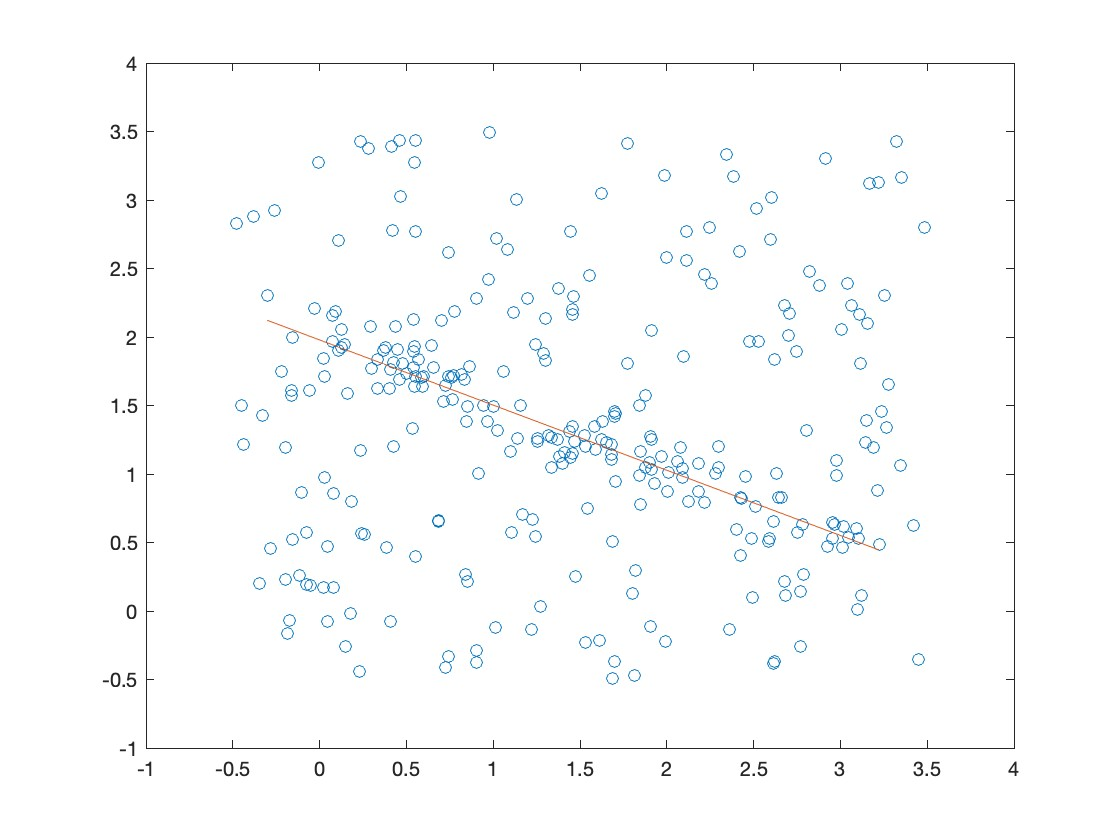
\includegraphics[width=5in]{figs/ransac_fit.jpg}}
    \caption{Figure showing the data points of $(x, y)$ coordinates as a scatter plot and a line model fitted using the RANSAC algorithm. This line was found with an error of 0.0928 based on inliers found from the algorithm.}
    \label{fig:line}
\end{figure} 